\newpage
\chapter{Appendix - Extra figures}

% Low episode training energy prediction
\begin{figure}[ht]
	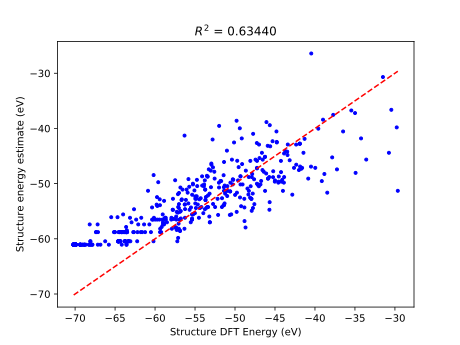
\includegraphics[width=\columnwidth]{graphics/energy_prediction_low_energy.pdf}
	\caption{This figure illustrates the possible problem that $\epsilon$-loop agents in ASLA may have encountered. The $\bm{\varepsilon}$ has been fitted using 500 structures from episodes up to 1000. It has then predicted the energy of 500 structures from episode 1001 and onwards, chosen randomly. Note that DFT energies below $\approx \SI{-62}{\electronvolt}$ will be assigned that energy. The energy range of the structures that are used for training seems to determine the prediction range. This could be a problem, since the structure filter works by sorted structures after predicted energies.}
	\label{fig:App_low_energy_predicts}
\end{figure}

\newpage
\thispagestyle{empty}

\begin{figure}
	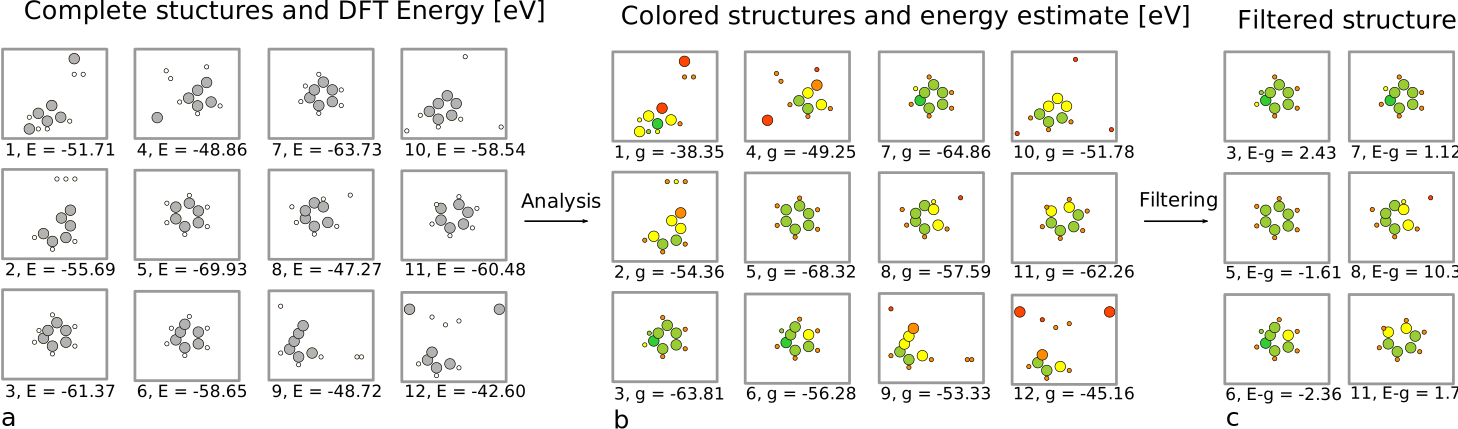
\includegraphics[angle=90, height=24cm]{graphics/filtering_demo.pdf}
	\caption{Enlarged version of figure \ref{fig:filtering}.}
	\label{fig:App_Filtering}
\end{figure}